%Chapter 3

\renewcommand{\thechapter}{3}

\chapter{UMER Apparatus and Diagnostics}
\label{ch:apparatus}

\section{UMER Layout}

UMER is laid out as a 36-sided polygon, comprised of 18 modular $20^o$ sections. Each section houses 2 dipole magnets over $10^o$ pipe bends and 4 quadrupole magnets in a FODO (focusing-defocusing) arrangement.

\section{UMER Beams}


	\subsection{Generation and Detection of Low-Current Beam}
	
	%%%%%%%%%%%%%%%%%%%%%%%%%%%%%%%%%%%%%%%%%%%%%%%%%%%%%%%%%%%%%%%%%%%%%%%%%%%%%%%%%%%%%%%%%%%%%%%%%%%%%%%%%%%%%%%%%%%%%%%%
	% IPAC 2015
	%%%%%%%%%%%%%%%%%%%%%%%%%%%%%%%%%%%%%%%%%%%%%%%%%%%%%%%%%%%%%%%%%%%%%%%%%%%%%%%%%%%%%%%%%%%%%%%%%%%%%%%%%%%%%%%%%%%%%%%%

\begin{figure}
\begin{center}
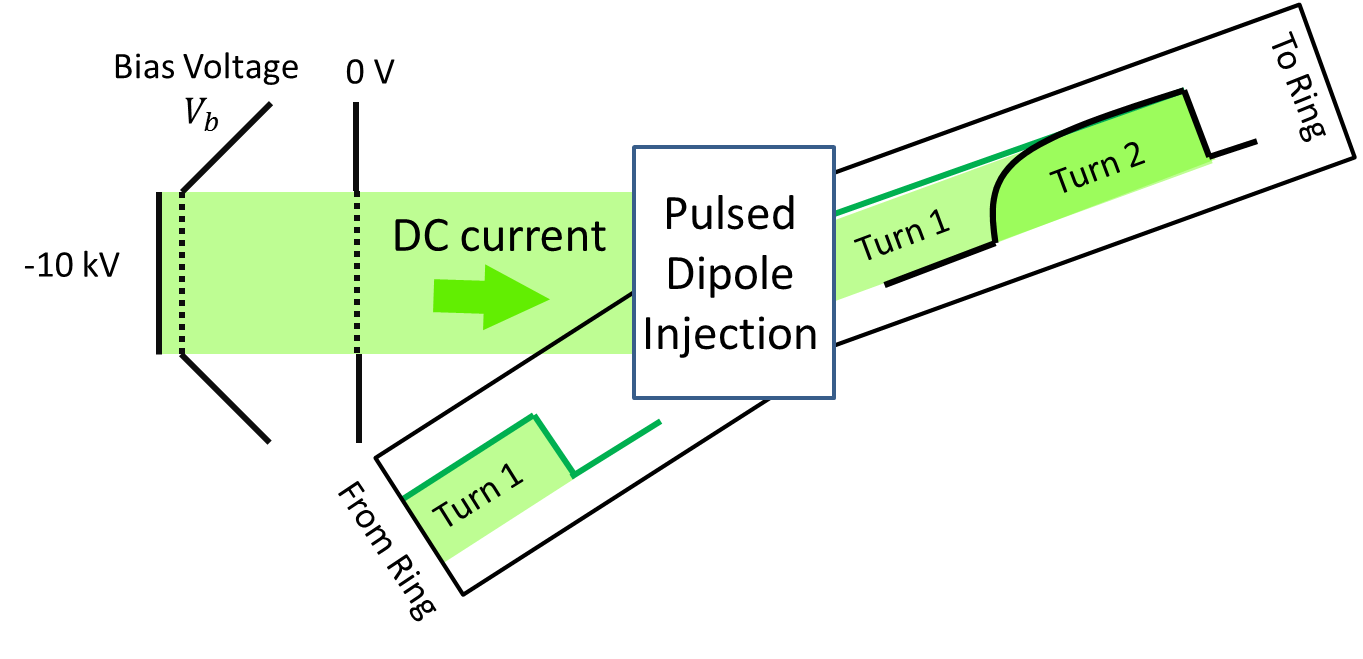
\includegraphics[width=\textwidth]{3.figures/DCbeam.png}
\end{center}
\renewcommand{\baselinestretch}{1}
\small\normalsize
\begin{quote}
\caption[]{Generation of variable current DC beam in UMER gun. Gate bias is lowered until DC current leaks through, pulse formation is done with injection dipole.}
\label{fig:DCbeamcartoon}
\end{quote}
\end{figure} 
\renewcommand{\baselinestretch}{2}
\small\normalsize
	
	
For experimental nonlinear dynamics, it is desirable to start with a primarily emittance dominated beam, with smaller space charge concentrations than the lower-limit UMER beam (0.6 mA, $\frac{\nu}{\nu_0}=0.85$), in order to isolate the space charge tune shift from the octupole tune shift. 
A nominally $50 \mu A$ beam was produced by reducing the cathode grid bias to allow leakage current and longitudinally gating the DC electron beam with the pulsed injector dipole. 
This resulted in a high-emittance, low current beam that maintained a DC signal for over 1000 turns, ultimately limited by the pulse length of the injection dipole. 
A low current, low emittance beam produced through photo-emission with a laser pulse is currently being explored as an additional UMER operating mode. 
%%%%%%%%%%%%%%%%%%%%%%%%%%%%%%%%%%%%%%%%%%%%%%%%%%%%%%%%%%%%%%%%%%%%%%%%%%%%%%%%%%%%%%%%%%%%%%%%%%%%%%%%%%%%%%%%%%%%%%%%
	
	
\section{Diagnostics}
\subsection{Beam Position Monitors}
\subsection{Wall Current Monitor}
\subsection{Transverse imaging}

\section{Measurement Techniques}
\subsection{Quadrupole-as-BPM technique}
\subsection{Tune Scans}	
	
	
\section{Lattice Configurations}
\subsection{FODO}

\begin{figure}[]
   \centering
   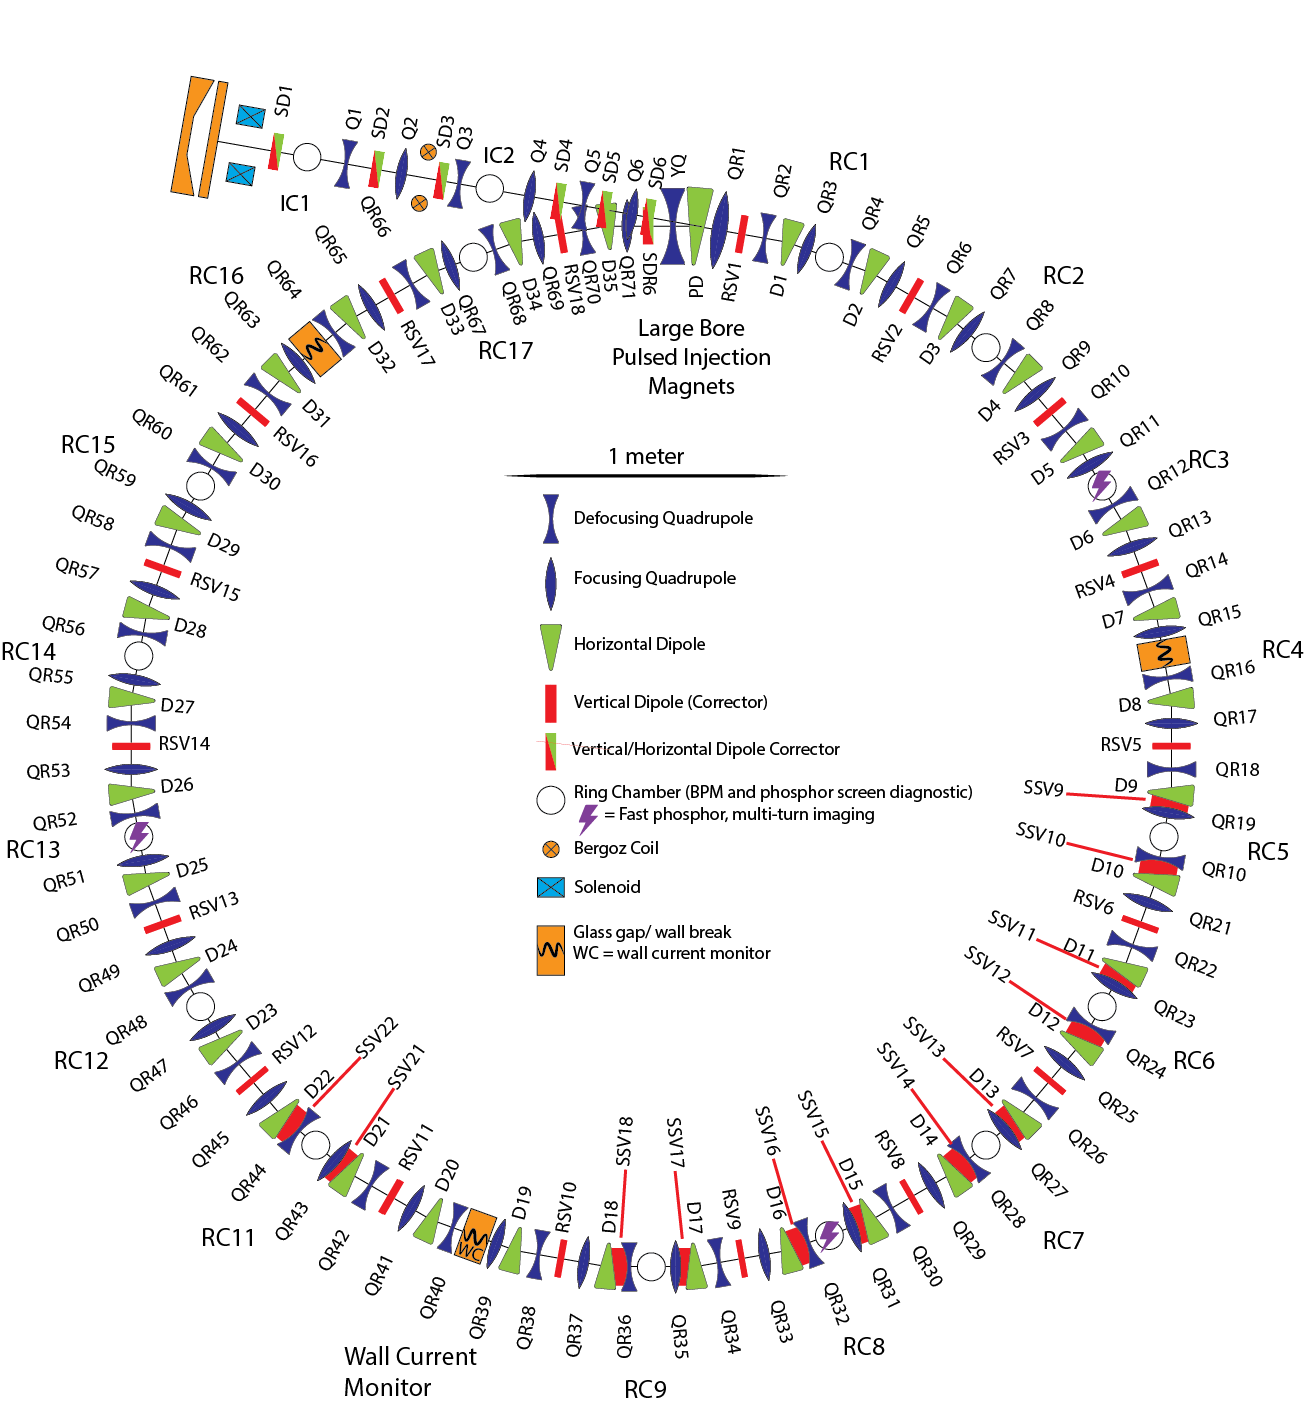
\includegraphics[width=\textwidth]{umer-diagram/full_ring.png}
   \caption{UMER ring, with all magnets labelled.}
   \label{fig:umerring}
\end{figure}

\subsection{Alternative FODO lattice}

\begin{figure}[]
%   \vspace*{-.5\baselineskip}
   \centering
   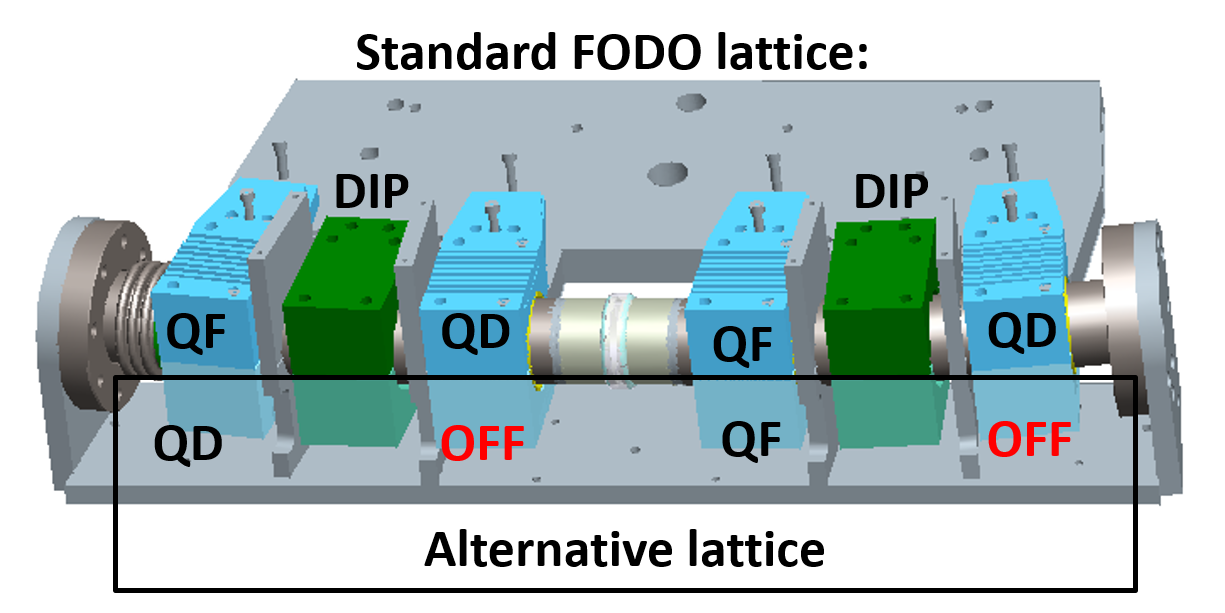
\includegraphics[width=0.7\textwidth]{6.figures/UMER_FODO.png}
   \caption{Two standard UMER FODO cells (blue quadrupoles and green dipoles). In the Alternatice lattice, the crossed quadrupoles are unpowered, leaving a vacancy for octupole elements.}
   \label{fig:FODOcell}
%   \vspace*{-\baselineskip}
\end{figure}

\begin{figure}[]
   \centering
   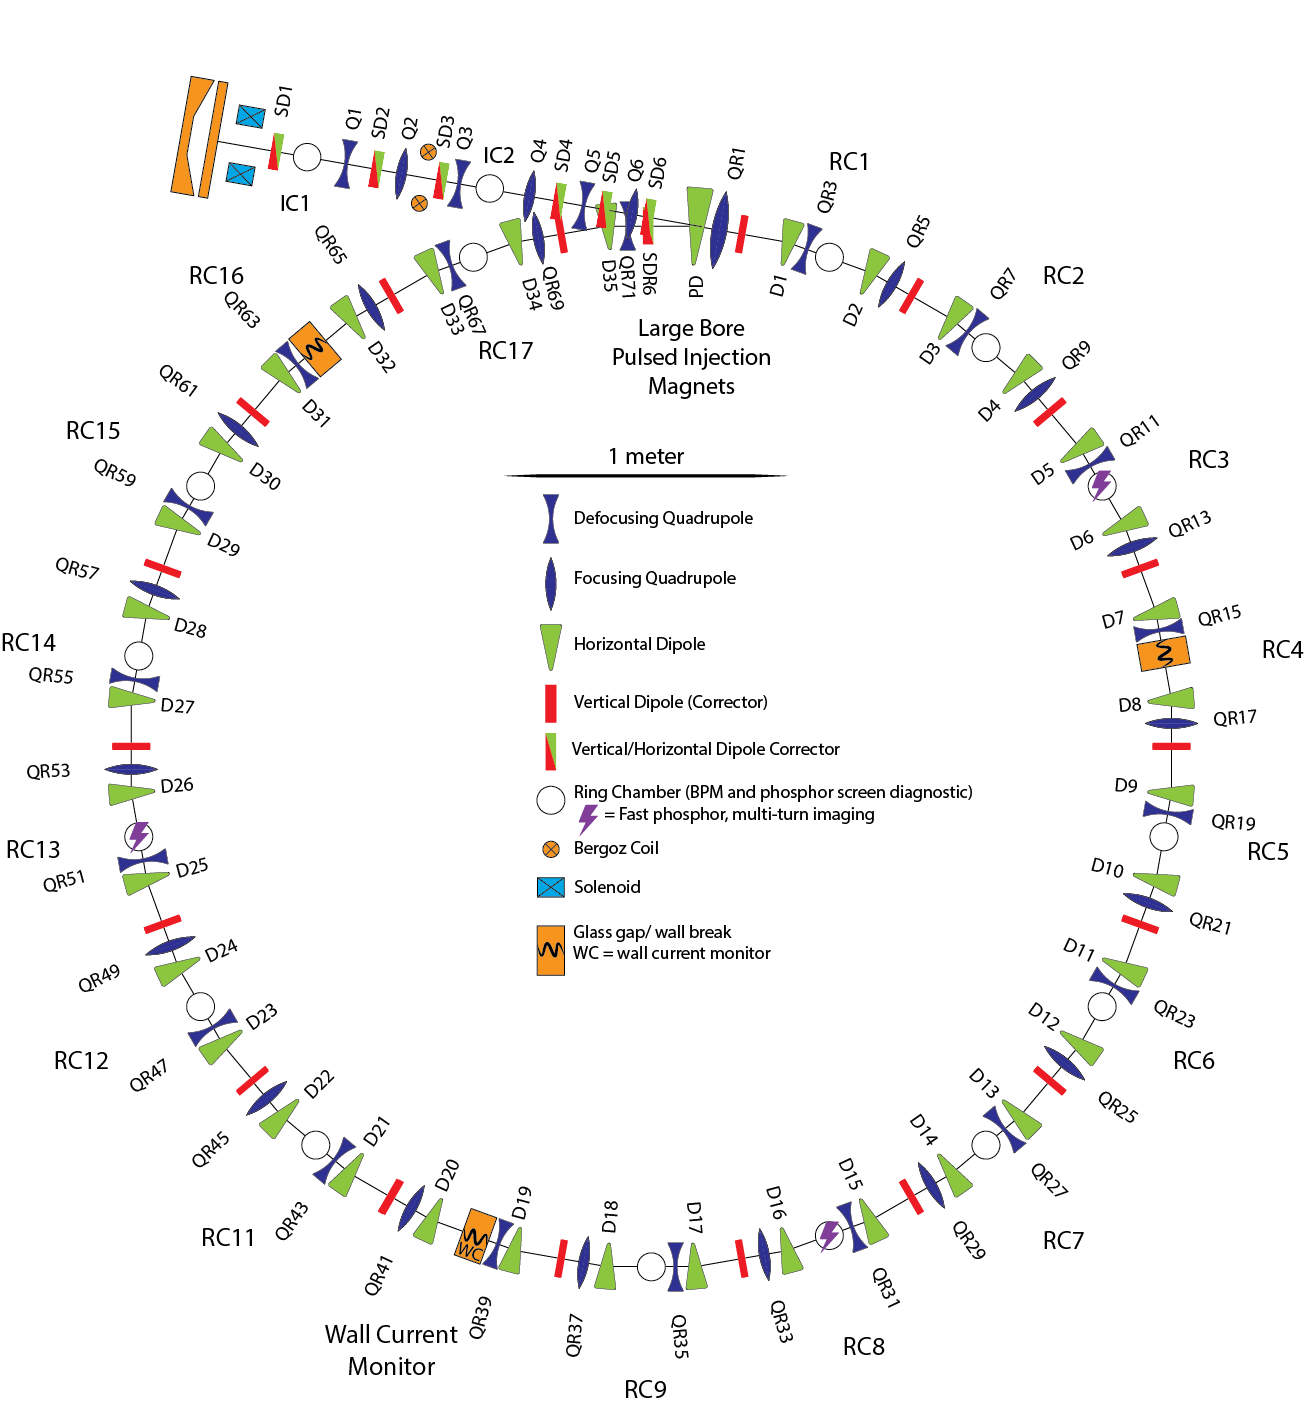
\includegraphics[width=\textwidth]{umer-diagram/altlat_full_ring.png}
   \caption{UMER ring in alternative lattice configuration.}
   \label{fig:altlatring}
\end{figure}

This configuration utilizes a mode of UMER operation known as the “alternative lattice” in which the total number of FODO cells in the ring is halved (by removing half of the quadrupoles).  The two lattices are illustrated in Fig. \ref{fig:FODOcell}. The nominal tune of the ring is also approximately halved, from $\nu \approx 6.7$ to $\approx 3.8$.






